
\newpage
\section{Evaluation}
Below we present our evaluation process, that place the prototype in the hands of real people, as recommended by validated guidelines \cite{article_mhealth, how_to_evaluate_tech_for_behaviour_change}.

Many people agree about the importance of designing systems for health and behaviour
change~\cite{article_mhealth, article_designing_for_healthy_lifestyles, article_designing_for_health_behaviour_change_hci}.
But each have varying opinions about how to evaluate these systems. Klasnja et al.~\cite{article_evaluate_tech_health_behaviour_change} focuses on system usability and does it meet the needs of users.
Whereas, Stawarz and Cox~\cite{article_designing_for_health_behaviour_change_hci} argue evaluating a system of this type requires information from other fields
to properly consider the systems effectiveness. The validated Behaviour Change Wheel Framework~\cite{article_behaviour_change_wheel} does just this.
Evaluating the system with validated behaviour change techniques from multiple domains. This project will use this framework to evaluate the chatbot with evaluation trials.
These will test the long-term effect and efficiency of the bot, with information from two fields of study, HCI and health psychology.

\subsection{Hypothesis}

Aslo talk about bot success as a third hypothesis

\subsection{Evaluation Trial Overview}
Evaluation trials are the final part of the Behaviour Change Wheel Framework~\cite{article_behaviour_change_wheel}.
HCI research that focuses on health interventions~\cite{article_mhealth}, demonstrates the importance of evaluation trials for evaluating mobile health systems.
These trials have three goals to test: objective-quantitative efficacy, subjective-qualitative feedback measures and real-world feedback about how the system is
utilised~\cite{article_evaluate_tech_health_behaviour_change}. I will conduct an evaluation trial for this project.\newline
\newline
The length of the trial will be based on two factors, the time needed to form a habit~\cite{article_how_habits_formed_modelling_habit_formation} and the results of a previous
habit formation trial~\cite{article_beyond_self_tracking_designing_apps}.
First, the number of repetitive days required for an action to be considered a habit varies based on the complexity of the action~\cite{article_how_habits_formed_modelling_habit_formation}.
Simple actions, such as drinking 2 glasses of water a day, can take a minimum of 18 days to form.
The suggested actions used for this project will be considered as simple, e.g. stretching for 30 seconds.
Second, a previous evaluation trial on habit-formation systems~\cite{article_how_habits_formed_modelling_habit_formation} showed an increase in habit automaticity after 4 weeks.
This project will mirror that timeframe.\newline
\newline
A 4-week evaluation trial will test the success of the chatbot by evaluating the tool and the effectiveness of each modality on users habit strength.
Chatbot interaction will be removed during the follow up study to test if users continue with the habit.
Participants will split into four groups, all groups will receive reminders, three groups will receive rewards each from a different modality,
and one group (control group) will not recieve any rewards.

\subsection{Testing Habit Strength}
Habit strength will be measured using a validated 12-question questionnaire that specifically looks at automaticity~\cite{article_habit_strength}.
Automaticity will also be measured using a validated subset of the questionnaire from~\cite{article_habit_strength} to test users habit behavioural
automaticity index~\cite{article_habit_measurement}. This will show the impact each modality has on habit automaticity and test the hypothesis.
Participants will fill out the questionnaires~\cite{article_habit_strength, article_habit_measurement} at three stages: half-way through the trial (at 2-weeks),
after the trial has finished and after the follow up trial.

\subsection{3-Week Trial}

Use everything from the paper section Method\newline
\newline
Breifly talk about Ethics approval, Kathys PHD 5.3.\newline
How participants were recruited, screenshots of all adverts\newline
Creating the adverts\newline
Photo of website\newline
Photo of Screens users would see, facebook post, website, get started, Setup (Link to full setup screens in appendix), recieving reminder message, reward, snoozed lots messages, end of study messages.\newline

Participants answered general demographic information as set up questions from the bot when they connected with it.

\begin{itemize}
\item \textit{Visual rewards}: Participants would receive a message that when tapped, would reveal a gif aimed at motivating them.
\item \textit{Auditory rewards}: Participants would receive a message that when tapped, would play a song aimed at motivating them.
\item \textit{Visual and auditory rewards}: Participants would receive a message that when tapped, would play a song and reveal a gif, aimed at motivating them.
\item \textit{No rewards (control group)}: Participants would only receive a confirmation message.
\end{itemize}

\begin{itemize}
  \item 'What is your gender?',
    \item 'How old are you?',
    \item 'Have you used habit tracking systems before? If did they work and what were they?',
    \item 'What habit do you want to track?',
    \item 'What existing routine would you like to use?',
    \item 'What time does that routine occur?',
    \item 'Would you like to be interviewed about your experience after the study?'.
\end{itemize}

\subsection{1-Week follow up trial}

Discussion of what the expected behaviour of the participant should be, bullet point list.\newline
Transcript/screenshot of end of study messages.\newline
Talk about asking for interview.

\subsection{Interview}

General overview of interview questions.\newline
Informal chat.\newline
Questions:
  - General questions firsts
  - Habit formation insight
  - Chabot interaction
  - Modality interaction
  - Are you still doing that habit?
  - Why did you pick that habit?
  - Do you want it back?


\section{Results}

General discussion about how the results were analysed. Technology used. Security.\newline
'Does giving users too much personalisation effect the study?'\newline


\subsection{Questions asked}

60 people made it through the website and pressed 'Get Started' in Facebook Messenger. These participants connected on these platforms: 25 browser, iOS 18 and Android 12.


54 people (90\%) started interacting with the bot and started the set-up. 39 people (65\%) completed the set-up. Out of these 39 people, 3 people just ignored the bot during the trial (didn't block the bot). Leaving 36 participants (66\%) that are consider active throughout and included in the final analysis.

The following questions are asked and answered.

\subsubsection*{What was the reward split for the remaining 36 participants:}

14 participants (39\%) were assigned the visual choice of rewards, but they also preferred to answer 'Not Yet' (72 times), when asked if they completed their habit.


\subsubsection*{How many people volunteered for an interview?}
28 participants


\subsubsection*{How were the modalities assign with the remaining people?}
Out of the remaining people who continued with the trial, the modalities were split across 36 people (100\%) into the following modalities: 14 people (39\%) visual, 9 people (25\%) visual and auditory, 7 people (19\%) auditory and 6 people (17\%) had no rewards (control group),


\subsubsection*{What modality had the most snoozes?}
Users with visual rewards (72 total) had the highest total number of snoozes, auditory was minimum (14). None had 55 total and visual and auditory had 45.

\subsubsection*{How many habits were completed?}
184 total habits were marked as completed, breakdown: Visual had 69, visual and auditory had 58, control group had 40 and auditory 17.

\subsubsection*{How many messages were sent?}
Users sent 1.1k messages to the bot with 3.8k total events, about 65 events average per user.

\subsubsection*{How many Facebook API calls were made?}
2,995 FB API calls, 319 errors

\subsubsection*{How many people dropped out/blocked bot?}

Throughout the study 24 people deleted the bot thread and 11 people turned off the bot (invalid participants anyway).

\subsubsection*{Did users like the bot?}
Yes: Well the number of snoozes over time decreased (chart), the number of habits completed per day increased (chart) and users streaks over time increased (chart). In addition, 36 people used it for 3-weeks. Also 31 participants actually completed a habit or marked one as not yet and 31 participants interacted with the bot at least once.

\subsubsection*{Were the rewards motivating?}
Not really: The graphs show that the number of snoozes for all modalities stays roughly the same, except for the control group which declines.


\subsubsection*{What was users habit context?}
31 people chose one of the contexts that were listed as examples, some with a slight change in before and after wording, e.g. before getting home from work, rather than after getting home from work. The remaining 5 people chose the following context: 'Having a snack', 'Sitting in bed', 'Early morning', 'during breakfast' and 'Before sleeping'.

Suggested habit contexts (by the bot):(todo insert table: morning, afternoon, evening habit context)

% Morning:
%   - waking up
%   - eating breakfast
%   - arriving at work

%   Afternoon:
%   - eating lunch
%   - leaving work

%   Evening:
%   - leaving work
%   - eating dinner
%   - getting ready for bed


\subsubsection*{When did people most say 'Not Yet'?}
Most people said 'Not Yet' in the morning (100 times), specifically mid (66) and late (27) morning.

%   Morning: 100: 7 (early) + 66 (mid) + 27 (late)
%   Afternoon: 54: 7 + 4 + 43
%   Evening: 32: 6 + 15 + 11


\subsubsection*{What was the participation gender breakdown?}
23 (64\%) Male, 11 (30\%) female, 2 (6\%) didn't say.


\subsubsection*{How many people previously used habit tracking systems before?}
7 people (19\%) used them before and 100\% of those people said they worked. They tracked habits such as 'Diet' (3 people), 'Exercise' (3 people), 'Deadlines' (2 people), 'Audiobook reading' (1), 'Weight' (1). These people all chose new habits that they hadn't listed that they had tracked before.


\subsubsection*{What was the participant age distribution?}
36 participants ages ranged from 18-63, (mean=27).

\subsubsection*{What is the comparison between the habits people chose and the number of habits people completed?}
Meditation was the most popular habit selected (12 people), followed by Press ups (8). Reading and writing were the least, only selected by 4 and 2 people respectively.

However, stretching (6 people) was the most completed habit (60 times) based on number of people who selected it: 10.0, (10.0 = 60/6). Followed by meditation (75 times), 6.25 (6.25 = 75/12). The least was the plank and reading with 3.75 (15/4) and 1.75 (7/4).

\subsubsection*{The number of habits completed v chosen habit breakdown}
Stretching had the most habits completed v chosen habit, 60 times marked as completed, 6 people chose stretching (10 = 60/6).

% Stretch: 10 (= 60 / 6 people chose stretching)
% Meditation: 6.25 (= 75 completed / 12 people)
% Writing: 5 (= 10 / 2 people)
% Press ups: 4 (= 32 / 8 people)
% Plank: 3.75 (= 15 / 4 people)
% Reading: 1.75 (= 7 / 4 people)


\subsubsection*{What is the highest streaked habit?}
Meditation had the most cumulative streak (17) followed by stretching (7 people).


\subsubsection*{How did recruiting participants go?}
The landing page (\url{www.harrymt.com/harryshabits}) was shared 7 (+ 4 by me) times. (todo <screenshots add>)


\subsubsection*{Was chatbot successful at running a trial?}
Did have a lot of issues, but did get a lot of data.


\subsubsection*{What is the correlation between reward and streaks?}
High streaks (streak over 10) had habits: meditation (total 135 streaks) and stretch (126 streaks). Rewards wise, VISUAL AND SOUND had the most streaks (126 combined), control group 75, then VISUAL (60)


\subsubsection*{What was the habit that lasted the longest?}
Stretch had the highest streak (18), meditation (15). However, overall, for all habits completed, meditation was the most streaked (269 combined), stretching (231 combined), then press ups (39) then plank (24)

\subsubsection*{Failed snoozes}
Visual and sound had the most number of failed snoozes (10, split over 6 people, 1 person had 5 failed snoozes). Then it was sound by 4.



\subsubsection{Automaticity}
Automaticity was used to measure the habit strength based on the reward used. SRBAI scores for each condition are presented in figure~\ref{fig:habit_4_item_survey1_v_survey2}.
Participants (N = 15, 41\%) completed the SRBAI (4-questions) at the end of the 3-week period. Most participants (N = 10, 27\%) completed the full 12-question SRHI 1-week later. Comparing the difference between the first questionnaire and the second: Auditory and visual rewards combined increased the most (9.4\%) from 32 SRBAI (mean = 16, SD = 2.828) to 35 SRBAI (mean = 17.5 (9.4\% increase), SD = 3.536). But, visual rewards had the highest score in both questionnaires, 73 SRBAI (mean = 14.6, SD = 4.336) for the first and 79 SRBAI (mean = 15.8, SD = 3.701) for the second (8.2\% increase). Finally, the auditory rewards had the least increase 15 SRBAI (mean = 15, SD = 0.0) to 16 SRBAI (mean = 15, SD = 0.0) (6.7\% increase) and the control group (without rewards) increased from 27 SRBAI (mean = 13.5, SD = 4.950) to 29 SRBAI (mean = 14.5, SD = 6.364) (7.4\% increase).

%         S 1   S 2   Increase
% NONE      27    29    7.4%
% AUDITORY    15    16    6.7%
% VISUAL    73    79    8.2%
% COMBINED    32    35    9.4%
% N: SD     4.950 6.364
% A: SD     0   0
% VISUAL:SD   4.336 3.701
% COMBINED:SD 2.828 3.536
% N: MEAN   13.5  14.5  7.4%
% A: MEAN   15    15    0.0%
% V: MEAN   14.6  15.8  8.2%
% C: MEAN   16    17.5  9.4%

\begin{figure}
  \centering
 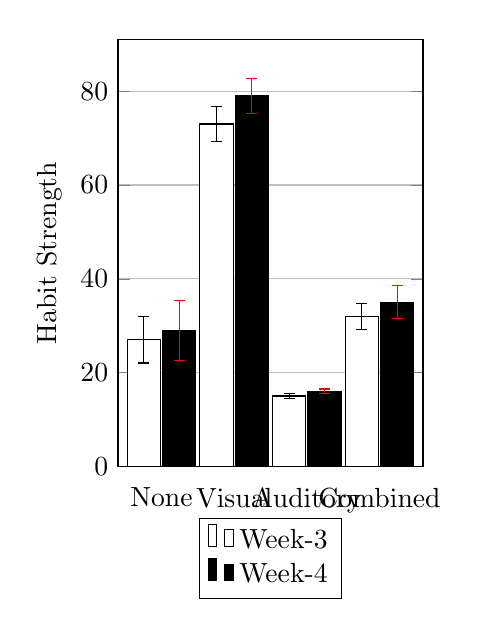
\begin{tikzpicture}
   \begin{axis}[
      width  = 0.45*\textwidth,
      height = 7cm,
      major x tick style = transparent,
      ybar=2*\pgflinewidth,
      bar width=12pt,
      ymajorgrids = true,
      symbolic x coords={None,Visual,Auditory,Combined},
      xtick = data,
      scaled y ticks = false,
      enlarge x limits=0.20,
      ymin=0,
      legend cell align=left,
      legend style={at={(0.5,-0.12)},anchor=north},
%       x label style={at={(axis description cs:0.5,-0.1)},anchor=north},
%       y label style={at={(axis description cs:-0.1,.5)},rotate=90,anchor=south},
%       xlabel={$u$ unemployment},
      ylabel={Habit Strength},
   ]
      \addplot[style={fill=white},error bars/.cd, y dir=both, y explicit]
          coordinates {
          (None, 27) += (0,4.950) -= (0,4.950)
          (Visual, 73) += (0,3.701) -= (0,3.701)
          (Auditory, 15) += (0,0.5) -= (0,0.5)
          (Combined, 32) += (0,2.828) -= (0,2.828)
          };

      \addplot[style={fill=black},error bars/.cd, y dir=both, y explicit,error bar style=red]
           coordinates {
           (None, 29) += (0,6.364) -= (0,6.364)
           (Visual, 79) += (0,3.701) -= (0,3.701)
           (Auditory, 16) += (0,0.5) -= (0,0.5)
           (Combined, 35) += (0,3.536) -= (0,3.536)
           };

      \legend{Week-3, Week-4}

  \end{axis}
  \end{tikzpicture}
  \caption{Comparing Habit strength verses reward type using the SRHI questionnaire for each modality.}~\label{fig:habit_4_item_survey1_v_survey2}
\end{figure}



\subsection{Other Results}
(NOTE: I am not sure if I should include any of these)

\subsubsection{What was users habit context?}
31 participants (86\%) chose one of the contexts that were listed as examples, some with a slight change in before and after wording, e.g. before getting home from work, rather than after getting home from work. The remaining 5 people chose the following context: 'Having a snack', 'Sitting in bed', 'Early morning', 'during breakfast' and 'Before sleeping'.

Suggested habit contexts (by the bot):(todo insert table: morning, afternoon, evening habit context)

Morning:
  - waking up
  - eating breakfast
  - arriving at work

  Afternoon:
  - eating lunch
  - leaving work

  Evening:
  - leaving work
  - eating dinner
  - getting ready for bed

  Morning: 100: 7 (early) + 66 (mid) + 27 (late)
  Afternoon: 54: 7 + 4 + 43
  Evening: 32: 6 + 15 + 11




\subsection*{Key results}

\subsubsection*{Compare the number of people dropped out verses Modality?}
(data here)
Visual: 7 people that had average 3.85 rewards and avg 2 snoozes\newline
Auditory: 2 people that had avg 2 rewards\newline
Visual and Auditory: 2 people that had an avg of 6.5 rewards.

%       Modality: # People | reward amount | Average Reward amount | Snoze amount | Avg snooze
%       VISUAL: 7 | 3, 1, 4, 4, 2, 12, 1 | 3.85 | 2, 5, 1, 0, 2 | 2
%       SOUND: 2 | 2, 2 | 2 | 0 | 0
%       VISUAL_AND_SOUND: 2 | 8, 5 | 6.5 | 6, 18 | 12

\subsubsection*{How many habits were completed, verses, modality type?}
VISUAL: Increasing. Rest: Decreasing (todo, compare with Habit survey). Then compare if users habit automaticity increased after using the bot / specific reward / habit questionnaire with result





\subsection{General Discussion}
General results analysed, with discussion. Lots of charts and graphs.



\subsection{Feedback}

- Feedback
  - Add a 'before' or 'after' option to avoid sythetic awkwardness (erasmo)
  - Liked music rewards.
  - If you tell the bot they haven't done their habit after their context, when they snooze it isnt going to be their context anymore!!! e.g. lunch at 5pm. The solution is to remove habit context from snoozed reminders.
  - TODO insert images\newline

Bot Reviews\url{https://developers.facebook.com/apps/319599908473430/messenger/bot-ratings/}


> I felt a bit like I was being nagged, and I don't like being nagged. The rewards were a bit odd. Would be nice to actually set a time to be asked about the habit.

> Interesting project but I did not ultimately feel motivated, the reminders became more of a chore than something I wanted to do.


\subsubsection*{Users issues they had}

\begin{itemize}
  \item x7 People tried to message to bot instead of using the quick replies
  \item x1 People tried to send multiple messages for free input, rather than all in a single message
  \item x1 Endless loop with different type
  \item x1 People tried to respond to the multiple messages with a thumb.
\end{itemize}

Development issues:

From the change to different database it was hard to test all aspects of the bot. For example the logic to send end of day messages was altered but not fixed.
Changed name of bot but did not update link on landing page
Removed FB messenger extensions but didn't remove Boolean value on reward button.
Enter negative age
Sometimes the reminder time is set to false. Maybe when people don't enter anything? Or if people abandon the setup, check a users conversation
The end of day reminders to decide if someone needed to be sent a 'unlucky' message was lost during the migration.
People reported multiple thanks messages / and messages in general.
If users interrupted the setup they restarted it. This annoyed users.
Double messages, j and Mum
Algo to auto assign modality has bad defaults ''
False in reminder times


\subsubsection*{Users feedback they gave in an unconventional way}
Feedback users gave when they just randomly messaged the bot.

\begin{itemize}
  \item Asked: What kind of thing are you looking to find out?
  \item Asked: 'Don't that will be annoying' when asked about being messaged every day
  \item Asked: 'Never' when asked about being messaged every day
  \item Asked: 'This is not working for me', got no response.
  \item Asked: 'Lame same band' when got same reward twice
  \item Asked: 'stop', then blocked the bot
  \item 1 user press a thumb to say they completed a habit
\end{itemize}


\subsection{Issues}
Issues with study results and general issues with implementation.

Discussion about the issues I had w the bot
\begin{figure}[H]
  \centering
  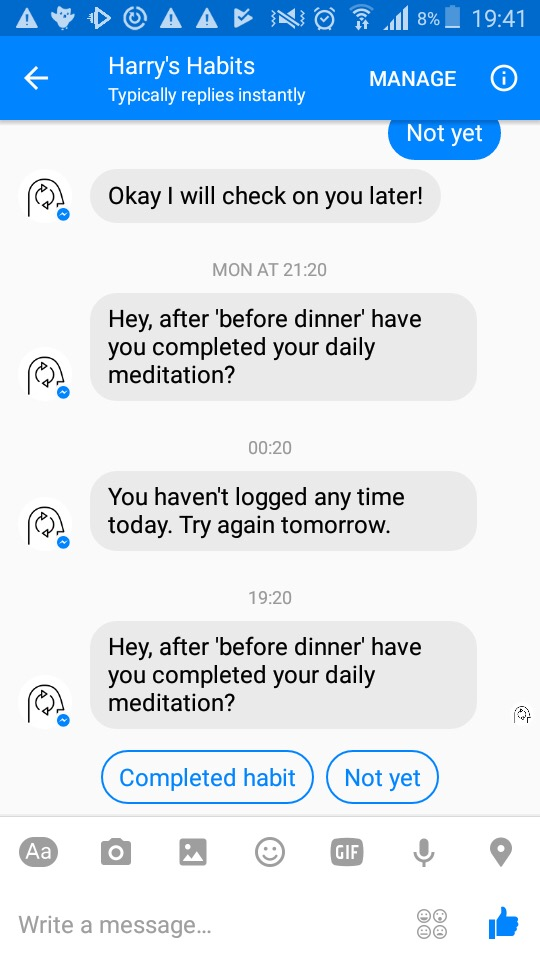
\includegraphics[width=2.1in]{../resources/feedback/after-before.jpg}
  \hspace{10px}
  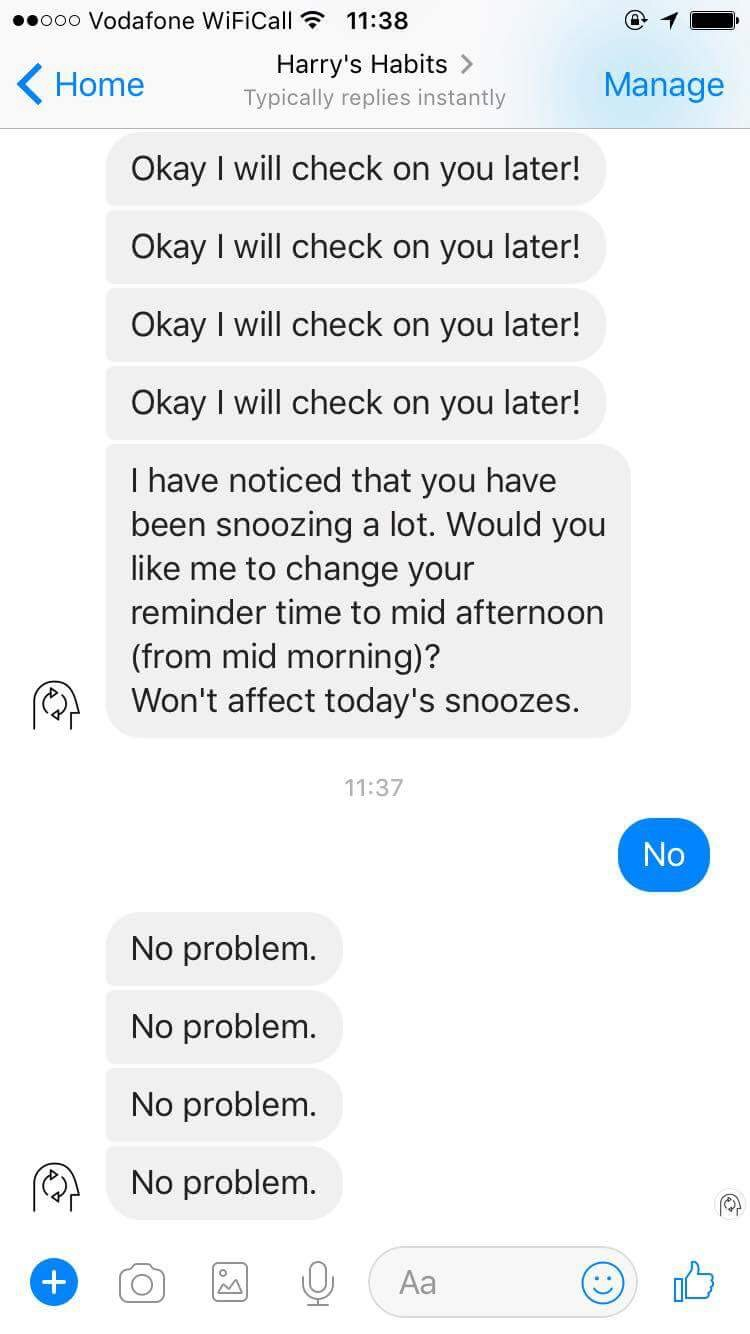
\includegraphics[width=2.1in]{../resources/feedback/double-messages.jpg}
  \caption{Example of 2 issues that occured, habit context using the word `after' and the bot sending multiple of the same messages.}
  \label{fig:study_bot_issues}
\end{figure}



\subsection{Summary}

Are the results even valid? What did we find out about the trail? Did we answer our research question?


